\chapter{Results}

Initial results were collected using the experimental platform. As described in
the experimental procedure chapter, various system topologies were tested with
the described packet loss rates. Tests using the experimental platform were run
as many as 40 times. The collected results have been divided into two sections:
SRC and SUC, the two delivery protocols used during testing.

The first minute of each test in the experimental test is discarded to remove
any transients in the test. The result is that while the tests were run for
ten minutes, the maximum result is 9 minutes of in group time.

\section{SRC}

\begin{figure}[!h]
\centering
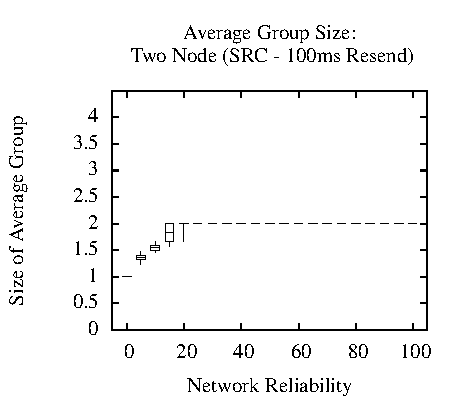
\includegraphics{2NODE-SRC-100-SIZE.pdf}
\caption{Average size of formed groups for two node system with 100ms resend time}
\label{fig:MGS-2NODE-100}
\end{figure}

\begin{figure}[!h]
\centering
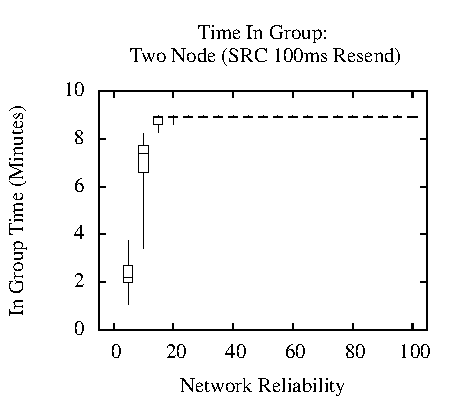
\includegraphics{2NODE-SRC-100-GROUP.pdf}
\caption{Average size of formed groups for two node system with 100ms resend time}
\label{fig:IGT-2NODE-100}
\end{figure}

The 100ms resend SRC test with two nodes can be considered a sort of a control.
These tests, pictured in Figures \ref{fig:MGS-2NODE-100} and
\ref{fig:IGT-2NODE-100}. This test highlights the excellent performance of the
SRC protocol.
